\documentclass[twocolumn]{article}

\usepackage[T1]{fontenc} % add special characters (e.g., umlaute)
\usepackage[utf8]{inputenc} % set utf-8 as default input encoding
\usepackage{amsmath,cite,url}
%\usepackage{ismir,amsmath,cite,url}
\usepackage{graphicx}
\usepackage{color}
\usepackage{parskip}
\usepackage{hyperref}


\usepackage{lineno}

\title{Leveraging LLMs for Retrieval Augmented Translation for English-to-Arabic Subtitles}


% Note: Please do NOT use \thanks or a \footnote in any of the author markup

% Single address
% To use with only one author or several with the same address
% ---------------
%\oneauthor
% {Names should be omitted for double-blind reviewing}
% {Affiliations should be omitted for double-blind reviewing}

% Two addresses
% --------------
%\twoauthors
%  {First author} {School \\ Department}
%  {Second author} {Company \\ Address}

% Three addresses
% --------------\input{ISMIR2021_paper.tex}

%\threeauthors
%{Mohamed Hannani } {Researcher }
%{Abdelhadi Soudi} {Professor}
%{Kristof Van Laerhoven} {Professor}

\author{
	Abdelhadi Soudi \\
	Professor
	\and
%	Kristof Van Laerhoven \\
%	Professor
%	\and
	Mohamed Hannani \\
	Researcher
}

\date{}  % Remove the date

% Four or more addresses
% OR alternative format for large number of co-authors
% ------------
%\multauthor
%{First author$^1$ \hspace{1cm} Second author$^1$ \hspace{1cm} Third author$^2$} { \bfseries{Fourth author$^3$ \hspace{1cm} Fifth author$^2$ \hspace{1cm} Sixth author$^1$}\\
	%  $^1$ Department of Computer Science, University , Country\\
	%$^2$ International Laboratories, City, Country\\
	%$^3$  Company, Address\\
	%{\tt\small CorrespondenceAuthor@ismir.edu, PossibleOtherAuthor@ismir.edu}
	%}

% For the author list in the Creative Common license, please enter author names. 
% Please abbreviate the first names of authors and add 'and' between the second to last and last authors.
%\def\authorname{F. Author, S. Author, and T. Author}

% Optional: To use hyperref, uncomment the following.
%\usepackage[bookmarks=false,pdfauthor={\authorname},pdfsubject={\papersubject},hidelinks]{hyperref}
% Mind the bookmarks=false option; bookmarks are incompatible with ismir.sty.

\sloppy % please retain sloppy command for improved formatting

\begin{document}
	

\maketitle

\begin{abstract}
While machine translation (MT) has made sign
icant progress in domain adaptation, achieving real-time adaptation for subtitles remains a formidable challenge. Large-scale language models (LLMs) have emerged as promising candidates for in-context learning. This study delves into the potential of in-context learning for real-time adaptive MT in the context of English-to-Arabic subtitles, with the utilization of the FAISS index for fuzzy match selection. Our experiments demonstrate the remarkable capacity of LLMs to adapt to in-domain content, surpassing traditional encoder-decoder MT models. Furthermore, we explore the integration of MT techniques, encompassing both robust encoder-decoder models and LLMs, with fuzzy matching. This integration reveals the potential to further elevate translation quality, a particularly valuable asset in the realm of English-to-Arabic subtitle translation, where language support may be limited. To validate our findings, we conducted extensive experiments focused on English-to-Arabic (EN-AR) subtitle translation.
	
\end{abstract}
%
\section{Introduction}\label{sec:introduction}

The ever-expanding landscape of natural language processing and machine translation has ushered in a new era of communication, significantly reducing linguistic divides and fostering cross-cultural understanding. While large language models, such as GPT, Llama 2, and the recently introduced Falcon have made remarkable strides in handling a wide range of language-related tasks, machine translation goes beyond mere word conversion. It entails the intricate task of preserving nuances, idioms, and the unique stylistic attributes that define human languages.

\begin{figure}
	\centering
	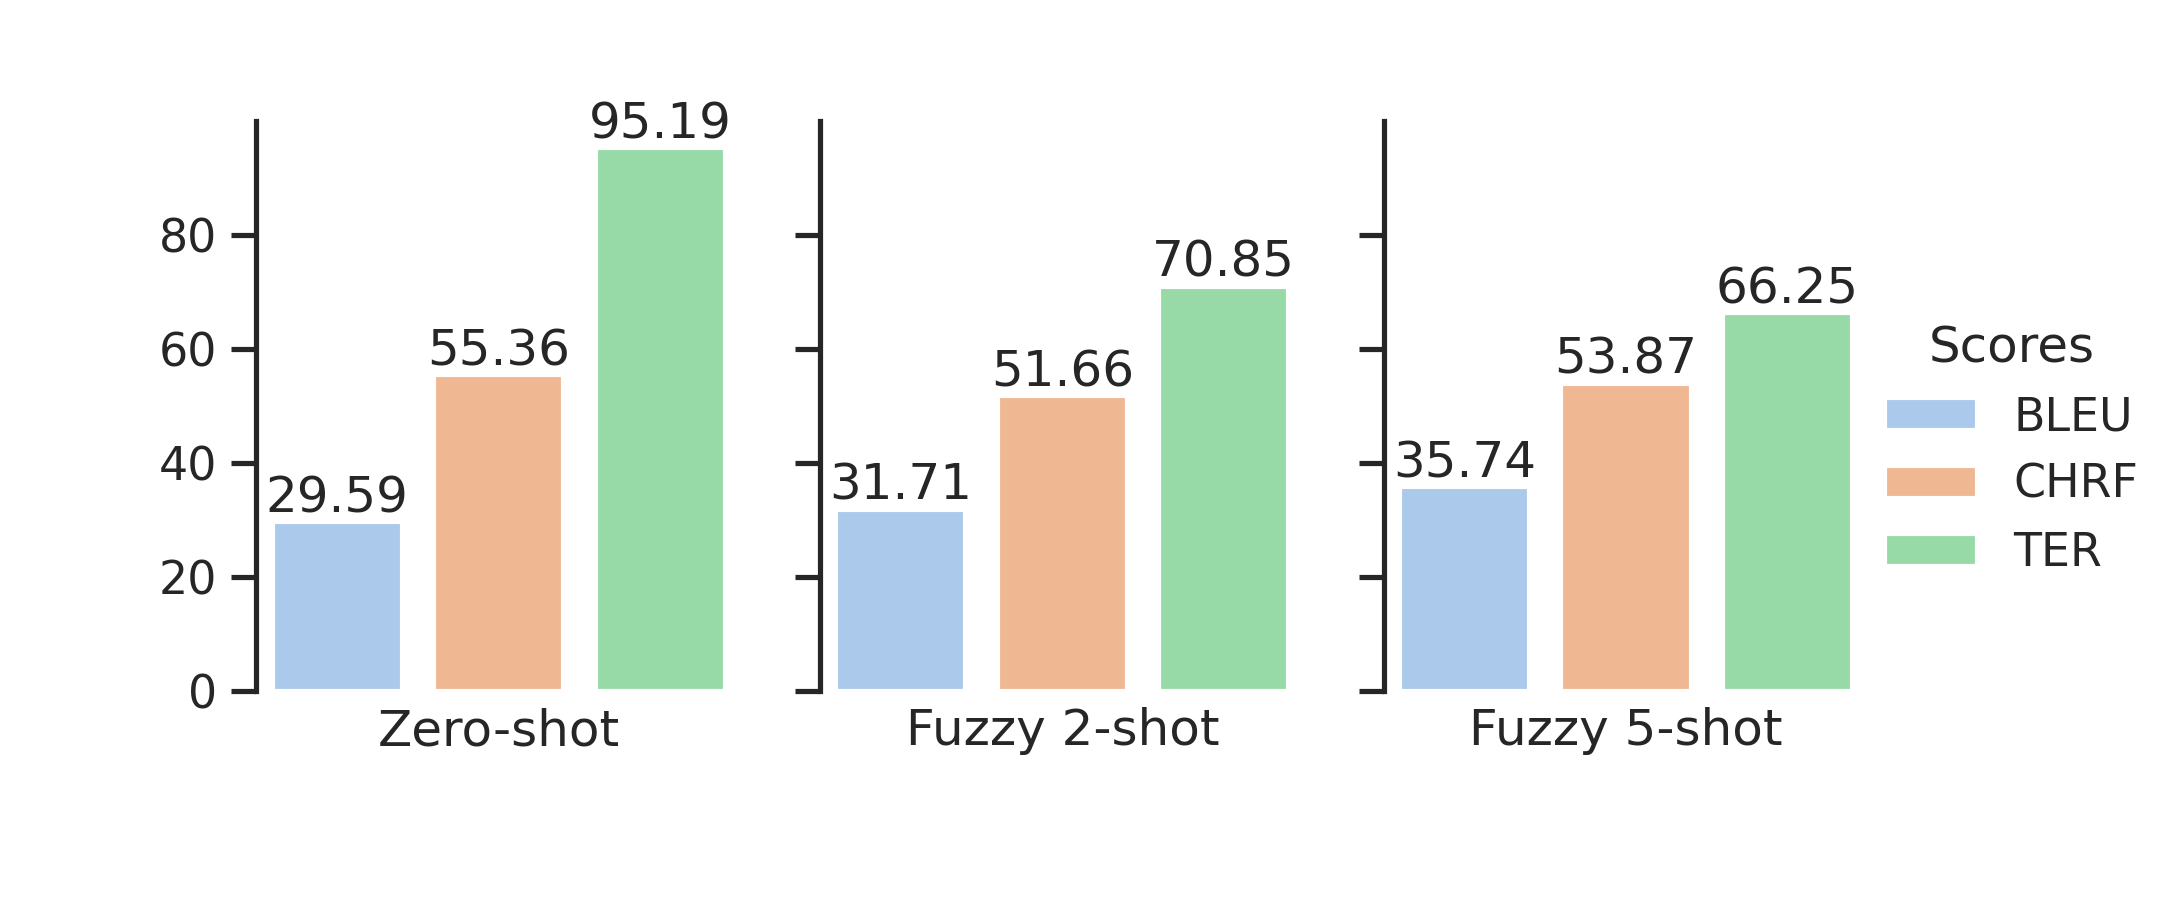
\includegraphics[width=\linewidth, ]{figs/Llama2_evaluation} % Adjust the height as needed
	\caption{ Evaluation results of Llama-2-70b-hf, with zero-shot, 2-shot and 5-shot fuzzy matches.}
	
	\label{llama_2_evaluation:duck}
\end{figure}


Language Language Models (LLMs), including but not limited to GPT-3\cite{brown2020language}, PaLM\cite{chowdhery2022palm}, Falcon\cite{penedo2023refinedweb}, and LLaMA\cite{touvron2023llama}, have been designed to predict the subsequent word in a sequence based on the context. Brown et al.\cite{brown2020language}; Ouyang et\cite{ouyang2022training} introduced the concept of "in-context learning" to describe a scenario where a pre-trained language model, during inference, assimilates specific input-output text generation patterns without the need for further fine-tuning. Their research highlighted that autoregressive LLMs like GPT-3 exhibit strong performance across diverse tasks, including zero-shot, one-shot, and few-shot in-context learning, all without necessitating updates to their weights. Instead of directly instructing the model to perform a particular task, input data can be enriched with relevant examples to facilitate the model's adaptation. The core principle of in-context learning revolves around learning from analogies embedded within demonstrations (Dong et al., 2022).


This brings us to the concept of adaptive translation, a paradigm aimed at enhancing machine translation by tailoring it to specific domains, genres, or styles. A key advantage of adaptive translation is its ability to achieve domain-specific translation goals without the resource-intensive processes of model training and fine-tuning. Our particular emphasis lies in harnessing the capabilities of Llama-2-70b-chat by Meta and GPT-3.5 Turbo by OpenAI with in-context samples.

This report delves into the intricacies of adapting machine translation to domain-specific requirements, utilizing a corpus of approximately 2,500 movie subtitles meticulously translated from English to Arabic. These subtitles encapsulate the nuances of cinematic language and provide a rich contextual source for our translation model. Prior to the inference phase, we leverage the Sentence-Transformer model to compute embeddings for these subtitles, streamlining the retrieval of similar sentences using the FAISS indexing system developed by Facebook. This approach enables us to construct contextually rich prompts, allowing Llama-2-70b-chat as well as GPT-3.5 Turbo to follow the stylistic cues present in domain-specific examples.

Prior studies have delved into the application of neural language models in Machine Translation (MT), encompassing few-shot in-context learning (Vilar et al., 2022) and venturing into the zero-shot paradigm (Wang et al., 2021). Additionally, other researchers have proposed leveraging Large Language Models (LLMs) to generate synthetic domain-specific data to facilitate MT domain adaptation (Moslem et al., 2022). Notably, recent research by Agrawal et al. (2022) and Zhang et al. (2023) has reaffirmed the critical role of in-context example selection in enhancing the quality of MT when employing LLMs.

The primary focus of this paper centers on exploring the capabilities of LLMs such as GPT-3.5, and Llama 2 in the context of real-time adaptive Machine Translation (MT). As depicted in Figure 1 for Llama 2, these LLMs exhibit the potential to enhance translation quality by adapting their output to align with the terminology and style found in previously validated translation pairs. Our particular areas of interest revolve around assessing the proficiency of these models in performing the following tasks without requiring additional training:


\begin{enumerate}
	\item Adapting newly generated translations to seamlessly match the terminology and style in the context
	
	\item Rectifying translations generated by more robust encoder-decoder MT systems using fuzzy matches to further enhance LLMs, and
	
	\item Emphasizing the significance of prompt engineering in improving the capabilities of Language Model Models (LLMs) by using relevant translation examples. 
	
\end{enumerate}

In the following sections, we provide a detailed account of dataset, methodology, experimental setup, results, and engage in a broader discussion of the implications of adaptive translation in the field of machine learning. 




\begin{figure}
	\centering
	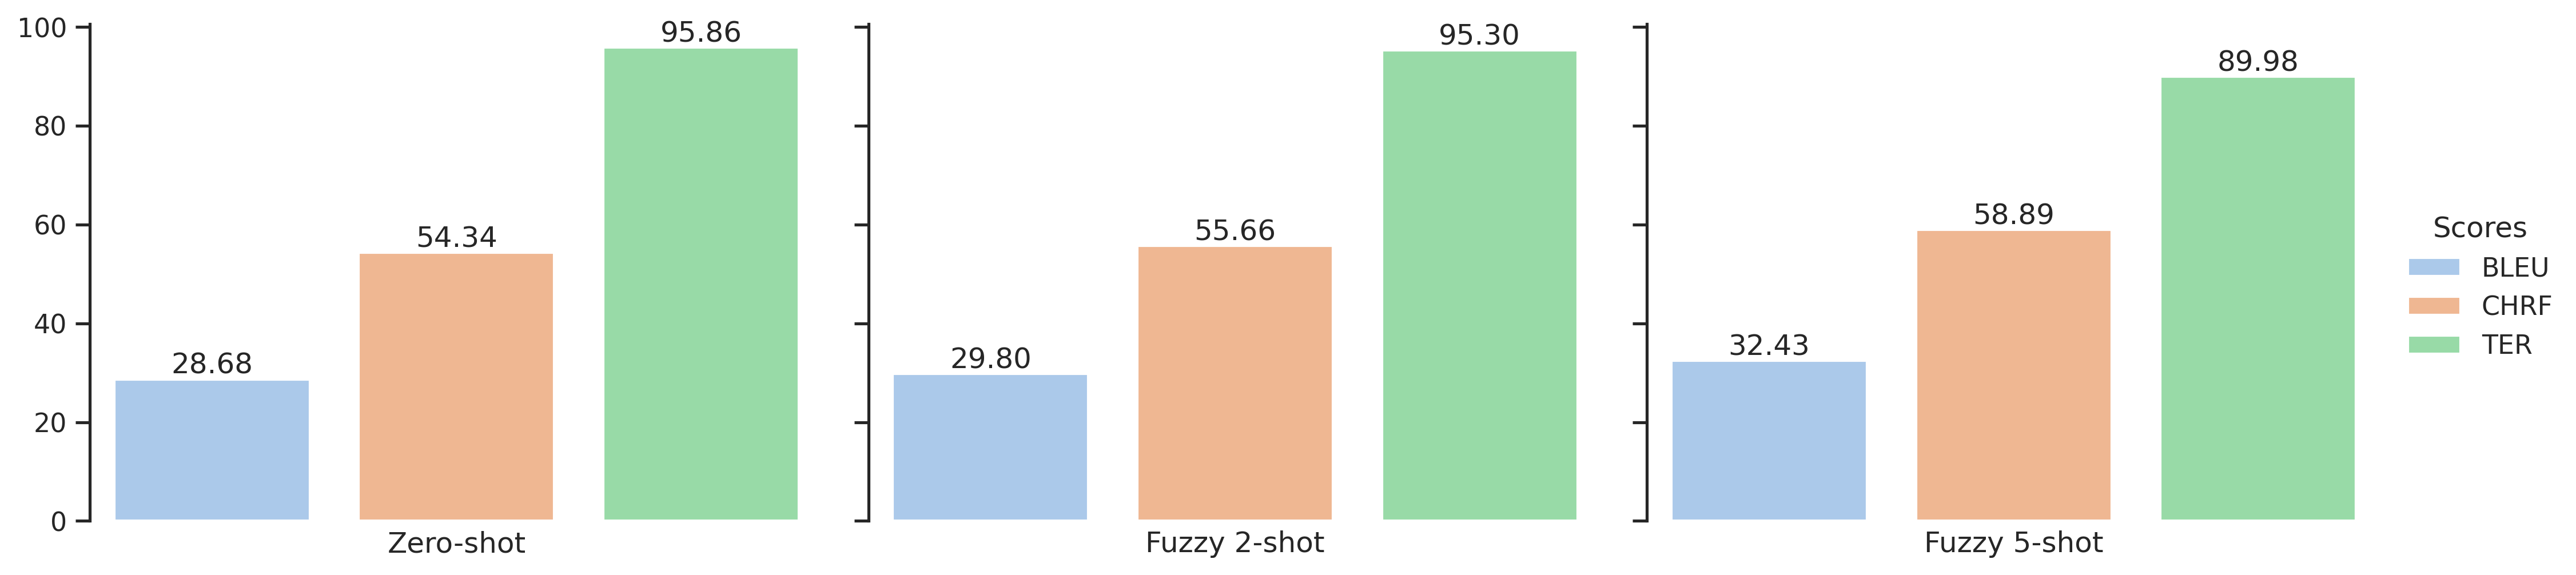
\includegraphics[width=\linewidth, ]{figs/chagpt_3_5_evaluation} % Adjust the height as needed
	\caption{ Evaluation results of GPT 3.5 Turbo, with zero-shot, 2-shot and 5-shot fuzzy matches.}
	
	\label{chagpt_3_5_evaluation:duck}
\end{figure}

\section{Dataset}
To build a robust translation model with domain-specific knowledge, we collected a dataset of approximately 1,500 movie subtitles that had been meticulously translated from English to Arabic. These subtitles were selected to represent a diverse range of cinematic language styles and contexts. 

The dataset was sourced from OpenSubtitles\cite{lison2016opensubtitles2016}, a well-known repository of subtitles
from a wide variety of movies and television shows. OpenSubtitles provides a valuable
resource for multilingual text data, making it suitable for training and evaluating
machine translation systems.


\section{Experimental setup}
In our experimental setup, we exclusively employed the OpenSubtitle dataset, specifically focusing on the English-to-Arabic translation task, comprising a total of 2,500 samples.

For our language model resources, we harnessed the power of two distinct Large Language Models (LLMs), namely GPT-3.5 Turbo via the OpenAI API and Llama 2 70b-hf through the Replica API.


\begin{table}[h]
	\centering
	\begin{tabular}{|c|c|c|c|}
		\hline
		\textbf{Parameters}  & \textbf{temperature} & \textbf{top\_p} & \textbf{n}\\
		\hline
		\textbf{Values}  & \textbf{0.7}  & \textbf{1}  & \textbf{1}\\
		\hline
	\end{tabular}
	\caption{GPT-3.5-turbo parameters with OpenAI API}
	\label{table:GPT_3.5_turbo_parameters_with_OpenAI_API}
\end{table}

In terms of parameterization, we maintained a consistent approach across the three translation tasks. We set respectively the 'top-p' parameter to 1  and applied a temperature value of 0.7 for GPT model Table \ref{table:GPT_3.5_turbo_parameters_with_OpenAI_API},  0.9 and 0.75 for Llama 2 model Table \ref{table:Llama_2_70b_chat_parameters}. 


\begin{table}[h]
	\centering
	\begin{tabular}{|c|c|c|c|}

		\hline
		\textbf{Parameters} & \textbf{temperature} & \textbf{top\_p} & \textbf{n}\\
		\hline
		\textbf{Values}  & \textbf{0.75}  & \textbf{0.9}  & \textbf{-}\\
		\hline
	\end{tabular}
	\caption{Llama 2 70b-chat parameters with Replicate}
	\label{table:Llama_2_70b_chat_parameters}
\end{table}


\section{Fuzzy Matches}

Machine translation (MT) plays a pivotal role in the professional and personal realms, yet its perfection remains an ongoing quest. One avenue toward elevating MT quality is the incorporation of fuzzy matches. These fuzzy matches comprise similar segments of previously approved translations stored within parallel datasets, commonly referred to as translation memories (TMs). Researchers have diligently explored the potential of fuzzy matches in bolstering MT quality and consistency \cite{knowles2018fuzzy,bulte2019fuzzy,xu2020forcing}.

For instance, the work of Knowles et al. (2018) revealed that the utilization of fuzzy matches could enhance the quality of neural MT (NMT) systems by up to 2 BLEU points \cite{knowles2018fuzzy}. Bulte and Tezcan (2019) extended this inquiry, demonstrating that fuzzy matches could enhance the consistency of MT systems, even in cases where these matches were not entirely precise \cite{bulte2019fuzzy}. In a recent investigation, Xu et al. (2020) delved into the prospect of compelling the translation of new sentence pairs to conform to the fuzzy matches found within the context dataset \cite{xu2020forcing}. They ascertained that this approach yielded improvements in MT quality, particularly for challenging sentences.

To unearth fuzzy matches, Xu et al. employed an embedding similarity-based retrieval method \cite{xu2020forcing}. This technique initiates by generating embeddings for each sentence within the TM. These embeddings represent sentences in dense numerical forms, encapsulating their semantic essence. Subsequently, the system retrieves fuzzy matches for a new sentence by identifying TM sentences with the most analogous embeddings. Previous research has established the superiority of embedding similarity-based retrieval over alternative methods like Edit Distance \cite{hosseini2020embedding}. For instance, Hosseini et al. (2020) demonstrated that this approach could augment fuzzy match recall by up to 10%.

Within the few-shot setting, the MT system is provided with a limited number of translated examples (e.g., 2 or 5) to assist in generating a translation for a new sentence. This stands in contrast to the zero-shot scenario where the MT system is solely equipped with the source sentence and language designations. Xu et al. uncovered that incorporating fuzzy matches through few-shot translation prompts could further heighten MT quality \cite{xu2020forcing}. This is attributed to fuzzy matches furnishing the MT system with additional insights into the desired translation's style and tone. He et al. (2022) introduced a novel method for incorporating fuzzy matches into NMT systems, employing a self-attention mechanism to discern the importance of each fuzzy match \cite{he2022incorporating}. This approach outperformed previous methodologies by up to 1 BLEU point across both high-resource and low-resource language pairs.

Furthermore, Wang et al. (2021) devised a more efficient and accurate embedding similarity-based retrieval algorithm \cite{wang2021more}. This algorithm expedites the retrieval of fuzzy matches while bolstering accuracy, consequently enhancing MT quality. Pham et al. (2021) investigated the role of fuzzy matches in ameliorating low-resource language translation \cite{pham2021fuzzy}. Their findings underscored the potential for leveraging fuzzy matches from high-resource language pairs to significantly enhance the translation of low-resource language pairs.

In tandem with these studies, there has been a burgeoning interest in leveraging fuzzy matches to enhance translations within specific domains, such as legal and medical contexts. For example, Li et al. (2023) proposed a novel approach harnessing fuzzy matches to refine the translation of legal documents \cite{li2023fuzzy}. Their method exhibited performance improvements of up to 2 BLEU points on a dataset comprising legal documents.

The above illustrations highlight the distinction between zero-shot and few-shot translation prompts. In the zero-shot scenario, only the source sentence and language specifications are provided, prompting the model to autonomously generate the translation. Conversely, the few-shot prompt incorporates translation examples, guiding the style of the generated output.

The results in Figure 1, Figure 2 highlight the remarkable performance difference between using Llama 2 70b-hf, as well as GPT 3.5 Turbo with 2-shot, 5-shot fuzzy matches and zero-shot translation. When employing fuzzy matches, translation quality metrics such as Blue and TER show substantial improvements, underlining the effectiveness of this approach in enhancing translation accuracy and fluency.

\begin{figure}
	\centering
	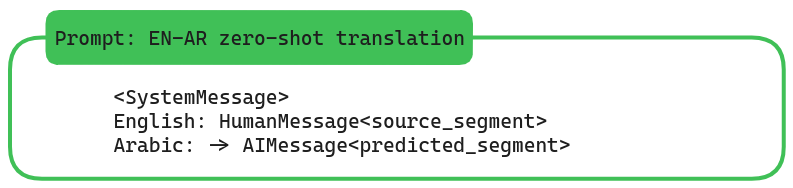
\includegraphics[width=\linewidth, ]{figs/prompt_zero_shot_translation} % Adjust the height as needed
	\caption{ Zero-shot translation prompt}
	
	\label{fig:duck_863}
\end{figure}

\begin{figure}
	\centering
	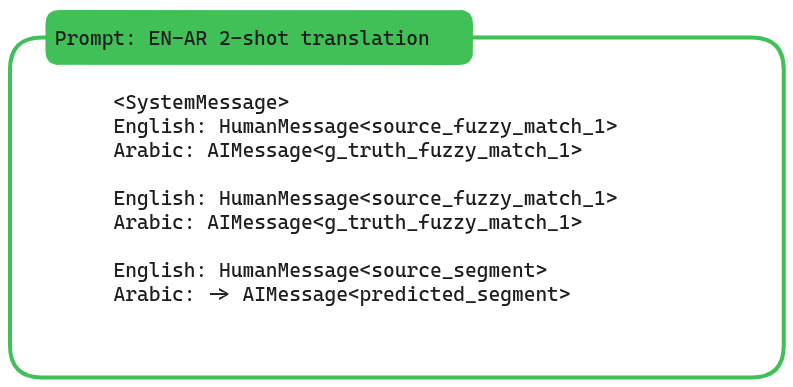
\includegraphics[width=\linewidth, ]{figs/prompt_two_shot_translation} % Adjust the height as needed
	\caption{ 2-shot translation prompt}
	
	\label{fig:duck_55}
\end{figure}


\section{Retrieval of Fuzzy matches}
To efficiently retrieve fuzzy matches for a given input sentence, we use the FAISS (Facebook AI Similarity Search) system. FAISS provides a variety of data structures and algorithms for efficient similarity search, and we have chosen to use the IndexFlatL2 index, which performs an exhaustive search of the index to find the nearest neighbors.

To generate the FAISS index, we first use the Sentence-Transformer model to generate embeddings for each sentence in our preprocessed dataset. Sentence embeddings are dense numerical representations of sentences that capture their semantic meaning and contextual nuances.


Once we have generated sentence embeddings for all of the sentences in our dataset, we can create the FAISS index. This involves the following steps:


\begin{enumerate}
	\item We load the sentence embeddings into FAISS,
	
	
	\item We configure the FAISS index with the desired parameters, such as the choice of index type and the dimensionality of the embeddings,
	
	
	\item We build the FAISS index for the whole corpus.
	
\end{enumerate}

Once the FAISS index has been built, we can use it to retrieve fuzzy matches for a given input sentence. To do this, we simply compute the cosine similarity between the input sentence embedding and all of the embeddings in the index. The sentences with the highest cosine similarities are the fuzzy matches for the input sentence.

We use the fuzzy matches to generate context-aware prompts for GPT-3.5 Turbo and Llama 2 70b-hf LLMs. These prompts provide GPT-3.5 Turbo with additional information about the desired translation, which can help it to generate more accurate and fluent translations.

FAISS and sentence embeddings allow for efficient and effective fuzzy match retrieval, which can be used to generate context-aware prompts for LLMs model to produce more accurate and fluent translations being context-aware.


\section{Prompt composition}

For each translation request, our approach leveraged the FAISS index to retrieve the top-k closest sentence embeddings from the domain-specific dataset. These retrieved sentences served as the foundation for constructing contextually rich prompts for the LLM model.


To facilitate prompt composition and enhance translation quality, we integrated Langchain into our system. Langchain is a versatile tool that enables the generation of coherent and domain-specific prompts. 

In our implementation, we utilized the following Langchain settings:

\textbf{SystemMessage:} We set the SystemMessage to: "Act like a good translator from English subtitles to Arabic subtitles. Translate the following English sentence into Arabic" for GPT3.5 Turbo and "Act like a good translator from English subtitles to Arabic subtitles. Translate the following English sentence to Arabic. Give me only the Arabic sentence, no Notes, and how to prounounce it". This SystemMessage template played a pivotal role in guiding the LLM model to follow the desired style and context for subtitle translation tasks. It acted as a foundational prompt template, providing a structured starting point for generating high-quality translations.
	

\textbf{HumanMessage} and \textbf{AIMessage}: Building upon the SystemMessage, we employed a combination of stacked HumanMessage and AIMessage. These messages were carefully crafted to maintain a conversational flow and ensure that the GPT model understood the user’s request.

The last \textbf{HumanMessage} in the sequence is the user’s sentence request, serving as the input for the translation task.


In the evaluation phase of the translation system, we leverage the above chat message format to interact with the GPT3.5 Turbo model effectively. Each translation request is encapsulated within a chat message, providing a structured way to communicate with the model. The chat message typically consists of a series of messages, including a SystemMessage, AIMessages, and a final UserMessage. The SystemMessage sets the context and instructs the model to perform as a skilled translator. AIMessages provide additional guidance, context, or clarifications as needed. The UserMessage encapsulates the user’s specific translation request, serving as the input for the model. By crafting messages in this manner, we ensure that the GPT model receives clear.

Worth the mention that the prompt composition of Llama 2 is the same as the GPT's one, but with some changes to the HumanMessage, Here the instruction tags that indicate the beginning ("[INST]") and end (`”/INST]”) of user input, wheras AIMessage was used as plain text without any instruction tags.


\section{Encoder-Decoder Models}
In this section, we aim to compare evaluation
results we obtained from MT encoder-decoder Transformer-based systems\cite{vaswani2017attention}, with those from GPT-3.5 and Llama 2 To this end, we translated our context dataset with Google Cloud Translation API. The results are detailed in Figure \ref{fig:google_transltation_evaluation}.

\begin{figure}
	\centering
	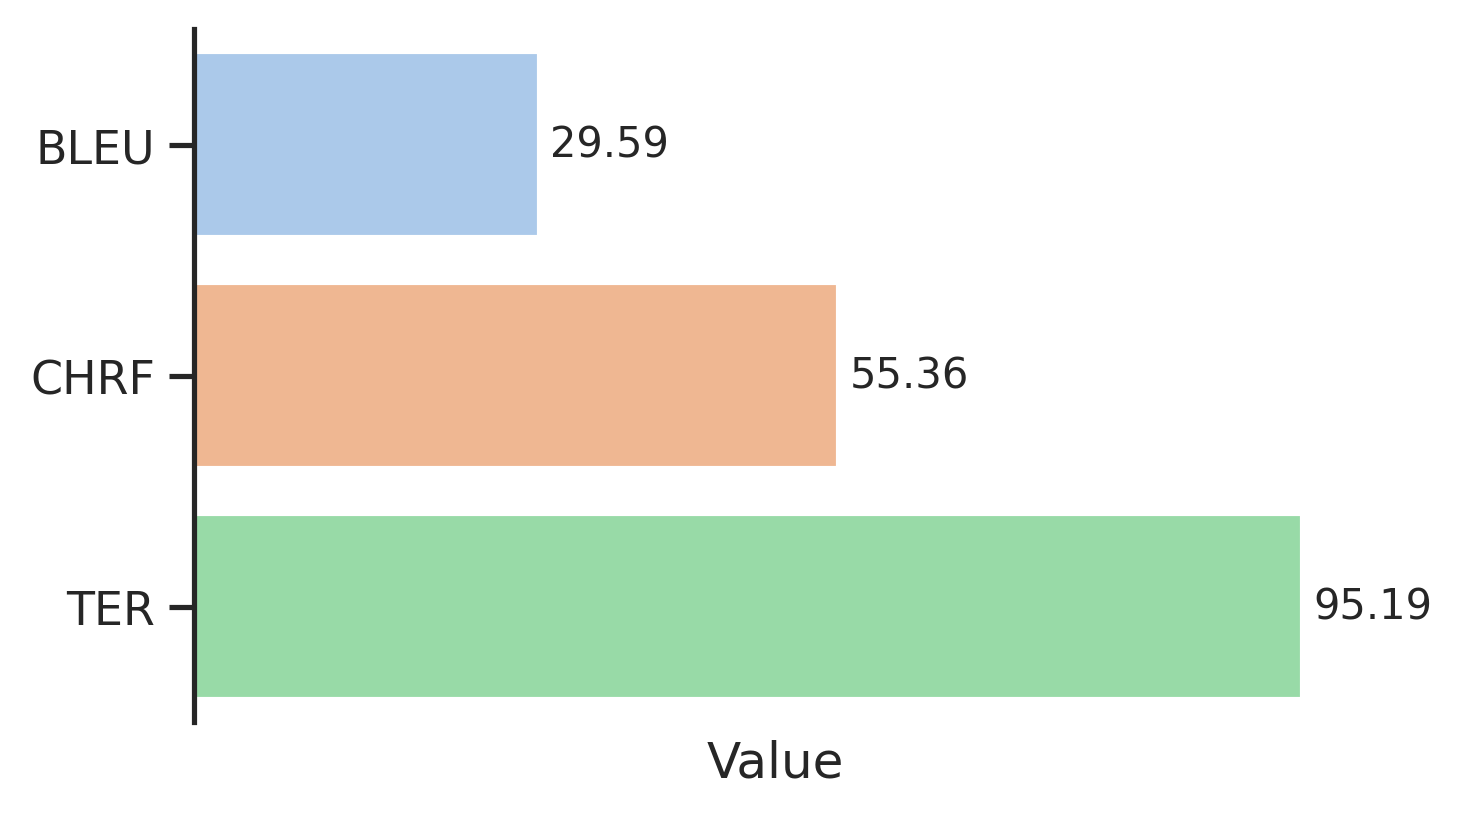
\includegraphics[width=\linewidth, ]{figs/Google_translate_api} % Adjust the height as needed
	\caption{ Google translation evaluation}
	
	\label{fig:google_transltation_evaluation}
\end{figure}

As demonstrated by Figure \ref{fig:google_transltation_evaluation}, We observe that for En-Ar subtitles, adaptive MT with or without fuzzy matches using GPT-3.5 and Llama 2 outperform Google Cloud Transalate API.

% For bibtex users:
\bibliography{ISMIRtemplate}

% For non bibtex users:
%\begin{thebibliography}{citations}
% \bibitem{Author:17}
% E.~Author and B.~Authour, ``The title of the conference paper,'' in {\em Proc.
	% of the Int. Society for Music Information Retrieval Conf.}, (Suzhou, China),
% pp.~111--117, 2017.
%
% \bibitem{Someone:10}
% A.~Someone, B.~Someone, and C.~Someone, ``The title of the journal paper,''
%  {\em Journal of New Music Research}, vol.~A, pp.~111--222, September 2010.
%
% \bibitem{Person:20}
% O.~Person, {\em Title of the Book}.
% \newblock Montr\'{e}al, Canada: McGill-Queen's University Press, 2021.
%
% \bibitem{Person:09}
% F.~Person and S.~Person, ``Title of a chapter this book,'' in {\em A Book
	% Containing Delightful Chapters} (A.~G. Editor, ed.), pp.~58--102, Tokyo,
% Japan: The Publisher, 2009.
%
%
%\end{thebibliography}
	
\end{document}